\documentclass[crop, tikz]{standalone}
\usepackage{tikz}

\usetikzlibrary{positioning}

\definecolor{echodrk}{HTML}{0099cc}
\definecolor{olivegreen}{rgb}{0,0.6,0}
\definecolor{camdrk}{RGB}{0,62,114}

\begin{document}
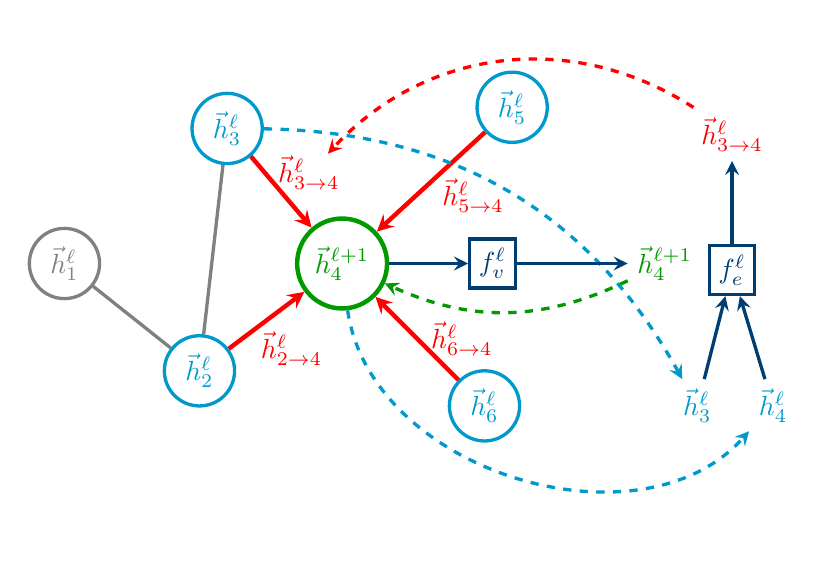
\begin{tikzpicture}
	\node[circle, gray, draw, very thick] (1) {$\vec{h}^\ell_1$};
	\node[circle, echodrk, draw, below right=2em and 3em of 1, very thick] (2) {$\vec{h}^\ell_2$};
	\node[circle, draw, echodrk, above right=3em and 4em of 1, very thick] (3) {$\vec{h}^\ell_3$};
	\node[circle, draw, olivegreen, right=7em of 1, ultra thick] (4) {$\vec{h}^{\ell+1}_4$};
	\node[circle, echodrk, draw, above right=3.5em and 4em of 4, very thick] (5) {$\vec{h}^\ell_5$};
	\node[circle, echodrk, draw, below right=3em and 3em of 4, very thick] (6) {$\vec{h}^\ell_6$};
		
	\draw[gray, very thick] (1) -- (2);
	\draw[gray, very thick] (2) -- (3);
	\draw[red, ultra thick, -stealth] (2) -- node[below, xshift=0.9em] (ll) {$\vec{h}_{2\rightarrow 4}^\ell$} (4);
	\draw[red, ultra thick, -stealth] (3) -- node[above,xshift=1em, inner sep=0em] (l1) {$\vec{h}_{3\rightarrow 4}^\ell$} (4);
	\draw[red,ultra thick, -stealth] (5) -- node[right, yshift=-0.5em] (lr) {$\vec{h}_{5\rightarrow 4}^\ell$} (4);
	\draw[red,ultra thick, -stealth] (6) -- node[right, xshift=0.1em] (lw) {$\vec{h}_{6\rightarrow 4}^\ell$} (4);
		
	\node[right=5.5em of 6, echodrk] (31) {$\vec{h}^\ell_3$};
	\node[right=1em of 31, echodrk] (41) {$\vec{h}^\ell_4$};
		
	\node[rectangle, draw, camdrk, very thick, above right=3em and -0.5em of 31] (F) {$f_e^\ell$};
		
	\node[above=3em of F, red] (34) {$\vec{h}^\ell_{3\rightarrow 4}$};
		
	\draw[very thick, camdrk, -stealth] (31) -- (F);
	\draw[very thick, camdrk, -stealth] (41) -- (F);
	\draw[very thick, camdrk, -stealth] (F) -- (34);
		
	\draw[very thick, -stealth, dashed, echodrk] (3) edge[bend left=30] (31);
	\draw[very thick, -stealth, dashed, echodrk] (4) edge[bend right=65] (41);
	\draw[very thick, -stealth, dashed, red] (34) edge[bend right=40] (l1);
		
	\node[right= of 4, camdrk, rectangle, draw, very thick] (G) {$f_v^\ell$};
	\node[right=4 em of G, olivegreen] (l11) {$\vec{h}^{\ell+1}_4$};
		
	\draw[-stealth, camdrk, very thick] (4) -- (G);
	\draw[-stealth, camdrk, very thick] (G) -- (l11);
		
	\draw[very thick, -stealth, dashed, olivegreen] (l11) edge[bend left=25] (4);
\end{tikzpicture}
\end{document}